\subsection{Problem}

\renewcommand{\theequation}{\theenumi}
\begin{enumerate}[label=\thesection.\arabic*.,ref=\thesection.\theenumi]
\numberwithin{equation}{enumi}
	\item Rain is falling vertically with a speed of $35ms^{-1}$. A woman rides a bicycle with a speed of $12ms^{-1}$ in east to west direction.What is the direction in which she should hold her umbrella?\\
The following python code computes the area of $\triangle$ABC in Fig.\ref{fig:qtwelve}.
	\begin{lstlisting}
	./codes/lines/q12.py
	\end{lstlisting}
	
	\solution At time t=0 let
\begin{align}
\vec{B} = \myvec{0\\0}
\end{align}
 denote the position of the woman. Since she rides her bicycle at $12ms^{-1}$ in east to west direction , her position at time t=1 is represented as 
\begin{align}
\vec{C} = \myvec{-12\\0}
\end{align}
. Let the position of a rain-droplet at time t=0 be 
\begin{align}
\vec{A} = \myvec{-12\\35}
\end{align}
. The drops which are falling a little ahead of the current position of the woman, will fall on her, because she moves in that direction.
To find the direction in which she should hold her umbrella, we need to find $\angle{CAB} =\theta$. 
\begin{multline}  
	\vec{AB = B-A} = \myvec{12\\-35}
	\\
	\vec{AC = C-A} = \myvec{0\\-35}
	\\
	\vec{AB}^T\vec{AC} = \norm{AB}\norm{AC}\cos{\theta}
	\\
	\cos{\theta} = \frac{35}{37}
	\\
	\theta = 18.93\degree 
\end{multline}
So the cyclist should hold the umbrella at 18.93$\degree$ to the vertical in the forward direction.

\begin{figure}[!ht]
	\centering
	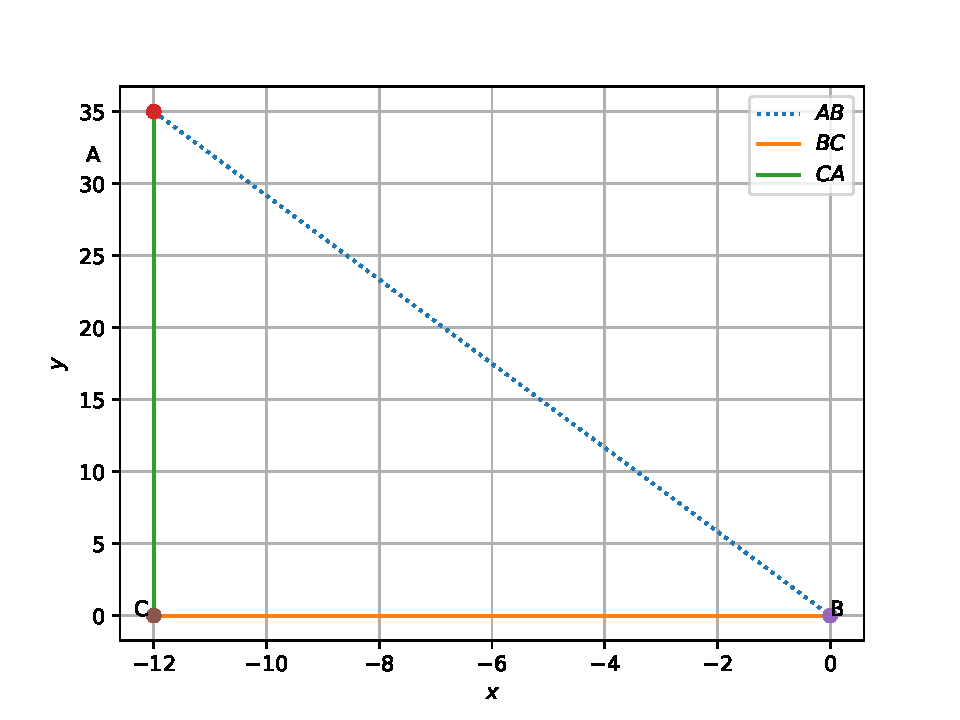
\includegraphics[width=\columnwidth]{./figs/lines/q12.pdf}
	\caption{Figure of Q.3.8.5}
	\label{fig:qtwelve}	
	\end{figure}
	


\end{enumerate}
